\chapter[16]{Семинар 16. Ввод--вывод данных. Поллинг. Программирование ввода--вывода}

Целью семинара является изучение взаимодействия процессора с устрокйствами ввода--вывода в режимет опроса состояния внешних устройств.

Изучение ведется на моделях внешних устройств, подключенных к эмулятору.
Примерный перечень вопросов:
\begin{enumerate}
    \item
    \item
\end{enumerate}

\begin{figure}[htbp]
    \centering
    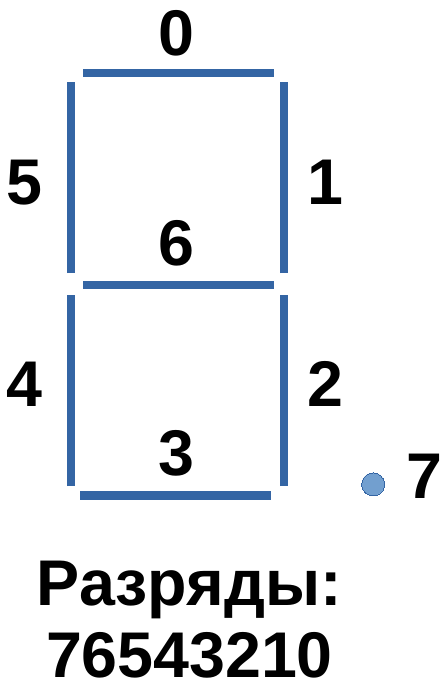
\includegraphics[width=0.3\textwidth]{img/digit-control.png}
    \caption{Отображение сегментов индикатора в данных, передаваемых устройству}
    \label{digit-control}
\end{figure}

\section{Домашнее задание}

